% !TEX TS-program = pdflatex
% !TEX encoding = UTF-8 Unicode
\documentclass[border=0mm]{standalone}
% packages
\usepackage{tikz}
\usetikzlibrary{patterns}
\usepackage{amsmath,amssymb}
\usepackage{bm}
\usepackage{pgfplots}
\pgfplotsset{compat=1.15}
% start document
\begin{document}
% generated by ROOT (CERN)
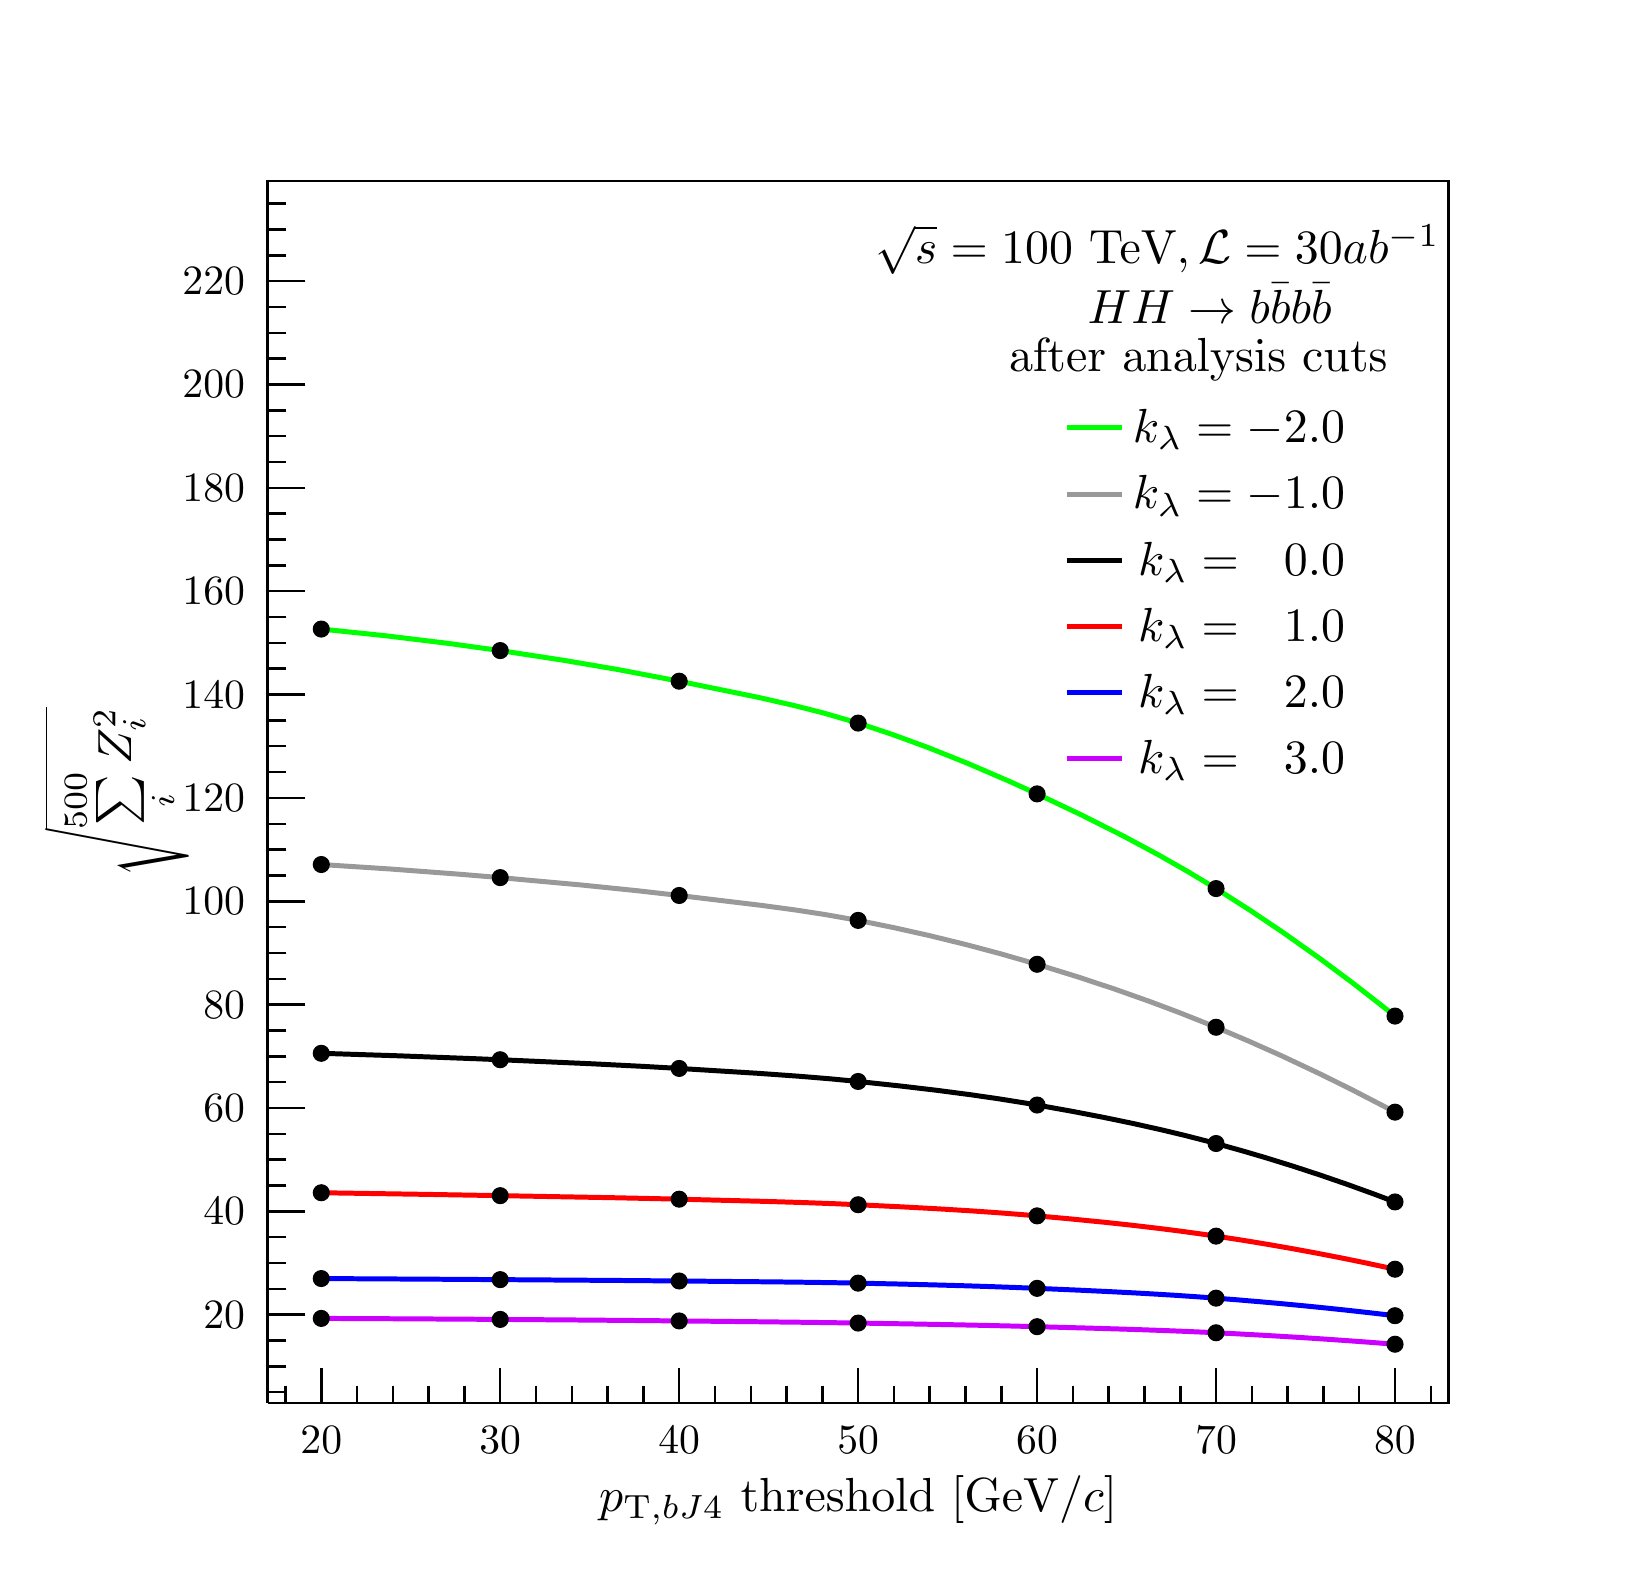
\begin{tikzpicture}
\pgfdeclareplotmark{cross} {
\pgfpathmoveto{\pgfpoint{-0.3\pgfplotmarksize}{\pgfplotmarksize}}
\pgfpathlineto{\pgfpoint{+0.3\pgfplotmarksize}{\pgfplotmarksize}}
\pgfpathlineto{\pgfpoint{+0.3\pgfplotmarksize}{0.3\pgfplotmarksize}}
\pgfpathlineto{\pgfpoint{+1\pgfplotmarksize}{0.3\pgfplotmarksize}}
\pgfpathlineto{\pgfpoint{+1\pgfplotmarksize}{-0.3\pgfplotmarksize}}
\pgfpathlineto{\pgfpoint{+0.3\pgfplotmarksize}{-0.3\pgfplotmarksize}}
\pgfpathlineto{\pgfpoint{+0.3\pgfplotmarksize}{-1.\pgfplotmarksize}}
\pgfpathlineto{\pgfpoint{-0.3\pgfplotmarksize}{-1.\pgfplotmarksize}}
\pgfpathlineto{\pgfpoint{-0.3\pgfplotmarksize}{-0.3\pgfplotmarksize}}
\pgfpathlineto{\pgfpoint{-1.\pgfplotmarksize}{-0.3\pgfplotmarksize}}
\pgfpathlineto{\pgfpoint{-1.\pgfplotmarksize}{0.3\pgfplotmarksize}}
\pgfpathlineto{\pgfpoint{-0.3\pgfplotmarksize}{0.3\pgfplotmarksize}}
\pgfpathclose
\pgfusepathqstroke
}
\pgfdeclareplotmark{cross*} {
\pgfpathmoveto{\pgfpoint{-0.3\pgfplotmarksize}{\pgfplotmarksize}}
\pgfpathlineto{\pgfpoint{+0.3\pgfplotmarksize}{\pgfplotmarksize}}
\pgfpathlineto{\pgfpoint{+0.3\pgfplotmarksize}{0.3\pgfplotmarksize}}
\pgfpathlineto{\pgfpoint{+1\pgfplotmarksize}{0.3\pgfplotmarksize}}
\pgfpathlineto{\pgfpoint{+1\pgfplotmarksize}{-0.3\pgfplotmarksize}}
\pgfpathlineto{\pgfpoint{+0.3\pgfplotmarksize}{-0.3\pgfplotmarksize}}
\pgfpathlineto{\pgfpoint{+0.3\pgfplotmarksize}{-1.\pgfplotmarksize}}
\pgfpathlineto{\pgfpoint{-0.3\pgfplotmarksize}{-1.\pgfplotmarksize}}
\pgfpathlineto{\pgfpoint{-0.3\pgfplotmarksize}{-0.3\pgfplotmarksize}}
\pgfpathlineto{\pgfpoint{-1.\pgfplotmarksize}{-0.3\pgfplotmarksize}}
\pgfpathlineto{\pgfpoint{-1.\pgfplotmarksize}{0.3\pgfplotmarksize}}
\pgfpathlineto{\pgfpoint{-0.3\pgfplotmarksize}{0.3\pgfplotmarksize}}
\pgfpathclose
\pgfusepathqfillstroke
}
\pgfdeclareplotmark{newstar} {
\pgfpathmoveto{\pgfqpoint{0pt}{\pgfplotmarksize}}
\pgfpathlineto{\pgfqpointpolar{44}{0.5\pgfplotmarksize}}
\pgfpathlineto{\pgfqpointpolar{18}{\pgfplotmarksize}}
\pgfpathlineto{\pgfqpointpolar{-20}{0.5\pgfplotmarksize}}
\pgfpathlineto{\pgfqpointpolar{-54}{\pgfplotmarksize}}
\pgfpathlineto{\pgfqpointpolar{-90}{0.5\pgfplotmarksize}}
\pgfpathlineto{\pgfqpointpolar{234}{\pgfplotmarksize}}
\pgfpathlineto{\pgfqpointpolar{198}{0.5\pgfplotmarksize}}
\pgfpathlineto{\pgfqpointpolar{162}{\pgfplotmarksize}}
\pgfpathlineto{\pgfqpointpolar{134}{0.5\pgfplotmarksize}}
\pgfpathclose
\pgfusepathqstroke
}
\pgfdeclareplotmark{newstar*} {
\pgfpathmoveto{\pgfqpoint{0pt}{\pgfplotmarksize}}
\pgfpathlineto{\pgfqpointpolar{44}{0.5\pgfplotmarksize}}
\pgfpathlineto{\pgfqpointpolar{18}{\pgfplotmarksize}}
\pgfpathlineto{\pgfqpointpolar{-20}{0.5\pgfplotmarksize}}
\pgfpathlineto{\pgfqpointpolar{-54}{\pgfplotmarksize}}
\pgfpathlineto{\pgfqpointpolar{-90}{0.5\pgfplotmarksize}}
\pgfpathlineto{\pgfqpointpolar{234}{\pgfplotmarksize}}
\pgfpathlineto{\pgfqpointpolar{198}{0.5\pgfplotmarksize}}
\pgfpathlineto{\pgfqpointpolar{162}{\pgfplotmarksize}}
\pgfpathlineto{\pgfqpointpolar{134}{0.5\pgfplotmarksize}}
\pgfpathclose
\pgfusepathqfillstroke
}
\definecolor{c}{rgb}{1,1,1};
\draw [color=c, fill=c] (0,0) rectangle (20,19.397);
\draw [color=c, fill=c] (3,1.9397) rectangle (18,17.4573);
\definecolor{c}{rgb}{0,0,0};
\draw [c,line width=0.9] (3,1.9397) -- (3,17.4573) -- (18,17.4573) -- (18,1.9397) -- (3,1.9397);
\definecolor{c}{rgb}{1,1,1};
\draw [color=c, fill=c] (3,1.9397) rectangle (18,17.4573);
\definecolor{c}{rgb}{0,0,0};
\draw [c,line width=0.9] (3,1.9397) -- (3,17.4573) -- (18,17.4573) -- (18,1.9397) -- (3,1.9397);
\draw [c,line width=0.9] (3,1.9397) -- (18,1.9397);
\draw [c,line width=0.9] (3.68182,2.37613) -- (3.68182,1.9397);
\draw [c,line width=0.9] (4.13636,2.15791) -- (4.13636,1.9397);
\draw [c,line width=0.9] (4.59091,2.15791) -- (4.59091,1.9397);
\draw [c,line width=0.9] (5.04545,2.15791) -- (5.04545,1.9397);
\draw [c,line width=0.9] (5.5,2.15791) -- (5.5,1.9397);
\draw [c,line width=0.9] (5.95455,2.37613) -- (5.95455,1.9397);
\draw [c,line width=0.9] (6.40909,2.15791) -- (6.40909,1.9397);
\draw [c,line width=0.9] (6.86364,2.15791) -- (6.86364,1.9397);
\draw [c,line width=0.9] (7.31818,2.15791) -- (7.31818,1.9397);
\draw [c,line width=0.9] (7.77273,2.15791) -- (7.77273,1.9397);
\draw [c,line width=0.9] (8.22727,2.37613) -- (8.22727,1.9397);
\draw [c,line width=0.9] (8.68182,2.15791) -- (8.68182,1.9397);
\draw [c,line width=0.9] (9.13636,2.15791) -- (9.13636,1.9397);
\draw [c,line width=0.9] (9.59091,2.15791) -- (9.59091,1.9397);
\draw [c,line width=0.9] (10.0455,2.15791) -- (10.0455,1.9397);
\draw [c,line width=0.9] (10.5,2.37613) -- (10.5,1.9397);
\draw [c,line width=0.9] (10.9545,2.15791) -- (10.9545,1.9397);
\draw [c,line width=0.9] (11.4091,2.15791) -- (11.4091,1.9397);
\draw [c,line width=0.9] (11.8636,2.15791) -- (11.8636,1.9397);
\draw [c,line width=0.9] (12.3182,2.15791) -- (12.3182,1.9397);
\draw [c,line width=0.9] (12.7727,2.37613) -- (12.7727,1.9397);
\draw [c,line width=0.9] (13.2273,2.15791) -- (13.2273,1.9397);
\draw [c,line width=0.9] (13.6818,2.15791) -- (13.6818,1.9397);
\draw [c,line width=0.9] (14.1364,2.15791) -- (14.1364,1.9397);
\draw [c,line width=0.9] (14.5909,2.15791) -- (14.5909,1.9397);
\draw [c,line width=0.9] (15.0455,2.37613) -- (15.0455,1.9397);
\draw [c,line width=0.9] (15.5,2.15791) -- (15.5,1.9397);
\draw [c,line width=0.9] (15.9545,2.15791) -- (15.9545,1.9397);
\draw [c,line width=0.9] (16.4091,2.15791) -- (16.4091,1.9397);
\draw [c,line width=0.9] (16.8636,2.15791) -- (16.8636,1.9397);
\draw [c,line width=0.9] (17.3182,2.37613) -- (17.3182,1.9397);
\draw [c,line width=0.9] (3.68182,2.37613) -- (3.68182,1.9397);
\draw [c,line width=0.9] (3.22727,2.15791) -- (3.22727,1.9397);
\draw [c,line width=0.9] (17.3182,2.37613) -- (17.3182,1.9397);
\draw [c,line width=0.9] (17.7727,2.15791) -- (17.7727,1.9397);
\draw [anchor=base] (3.68182,1.2996) node[scale=1.50669, color=c, rotate=0]{20};
\draw [anchor=base] (5.95455,1.2996) node[scale=1.50669, color=c, rotate=0]{30};
\draw [anchor=base] (8.22727,1.2996) node[scale=1.50669, color=c, rotate=0]{40};
\draw [anchor=base] (10.5,1.2996) node[scale=1.50669, color=c, rotate=0]{50};
\draw [anchor=base] (12.7727,1.2996) node[scale=1.50669, color=c, rotate=0]{60};
\draw [anchor=base] (15.0455,1.2996) node[scale=1.50669, color=c, rotate=0]{70};
\draw [anchor=base] (17.3182,1.2996) node[scale=1.50669, color=c, rotate=0]{80};
\draw (10.5,0.698292) node[scale=1.7299, color=c, rotate=0]{$p_{\text{T},bJ4} \text{~threshold} ~[\text{GeV}/c]$};
\draw [c,line width=0.9] (3,1.9397) -- (3,17.4573);
\draw [c,line width=0.9] (3.48,3.05906) -- (3,3.05906);
\draw [c,line width=0.9] (3.24,3.3872) -- (3,3.3872);
\draw [c,line width=0.9] (3.24,3.71533) -- (3,3.71533);
\draw [c,line width=0.9] (3.24,4.04347) -- (3,4.04347);
\draw [c,line width=0.9] (3.48,4.37161) -- (3,4.37161);
\draw [c,line width=0.9] (3.24,4.69975) -- (3,4.69975);
\draw [c,line width=0.9] (3.24,5.02788) -- (3,5.02788);
\draw [c,line width=0.9] (3.24,5.35602) -- (3,5.35602);
\draw [c,line width=0.9] (3.48,5.68416) -- (3,5.68416);
\draw [c,line width=0.9] (3.24,6.0123) -- (3,6.0123);
\draw [c,line width=0.9] (3.24,6.34043) -- (3,6.34043);
\draw [c,line width=0.9] (3.24,6.66857) -- (3,6.66857);
\draw [c,line width=0.9] (3.48,6.99671) -- (3,6.99671);
\draw [c,line width=0.9] (3.24,7.32485) -- (3,7.32485);
\draw [c,line width=0.9] (3.24,7.65298) -- (3,7.65298);
\draw [c,line width=0.9] (3.24,7.98112) -- (3,7.98112);
\draw [c,line width=0.9] (3.48,8.30926) -- (3,8.30926);
\draw [c,line width=0.9] (3.24,8.63739) -- (3,8.63739);
\draw [c,line width=0.9] (3.24,8.96553) -- (3,8.96553);
\draw [c,line width=0.9] (3.24,9.29367) -- (3,9.29367);
\draw [c,line width=0.9] (3.48,9.62181) -- (3,9.62181);
\draw [c,line width=0.9] (3.24,9.94994) -- (3,9.94994);
\draw [c,line width=0.9] (3.24,10.2781) -- (3,10.2781);
\draw [c,line width=0.9] (3.24,10.6062) -- (3,10.6062);
\draw [c,line width=0.9] (3.48,10.9344) -- (3,10.9344);
\draw [c,line width=0.9] (3.24,11.2625) -- (3,11.2625);
\draw [c,line width=0.9] (3.24,11.5906) -- (3,11.5906);
\draw [c,line width=0.9] (3.24,11.9188) -- (3,11.9188);
\draw [c,line width=0.9] (3.48,12.2469) -- (3,12.2469);
\draw [c,line width=0.9] (3.24,12.575) -- (3,12.575);
\draw [c,line width=0.9] (3.24,12.9032) -- (3,12.9032);
\draw [c,line width=0.9] (3.24,13.2313) -- (3,13.2313);
\draw [c,line width=0.9] (3.48,13.5595) -- (3,13.5595);
\draw [c,line width=0.9] (3.24,13.8876) -- (3,13.8876);
\draw [c,line width=0.9] (3.24,14.2157) -- (3,14.2157);
\draw [c,line width=0.9] (3.24,14.5439) -- (3,14.5439);
\draw [c,line width=0.9] (3.48,14.872) -- (3,14.872);
\draw [c,line width=0.9] (3.24,15.2001) -- (3,15.2001);
\draw [c,line width=0.9] (3.24,15.5283) -- (3,15.5283);
\draw [c,line width=0.9] (3.24,15.8564) -- (3,15.8564);
\draw [c,line width=0.9] (3.48,16.1846) -- (3,16.1846);
\draw [c,line width=0.9] (3.48,3.05906) -- (3,3.05906);
\draw [c,line width=0.9] (3.24,2.73092) -- (3,2.73092);
\draw [c,line width=0.9] (3.24,2.40278) -- (3,2.40278);
\draw [c,line width=0.9] (3.24,2.07465) -- (3,2.07465);
\draw [c,line width=0.9] (3.48,16.1846) -- (3,16.1846);
\draw [c,line width=0.9] (3.24,16.5127) -- (3,16.5127);
\draw [c,line width=0.9] (3.24,16.8408) -- (3,16.8408);
\draw [c,line width=0.9] (3.24,17.169) -- (3,17.169);
\draw [anchor= east] (2.9,3.05906) node[scale=1.50669, color=c, rotate=0]{20};
\draw [anchor= east] (2.9,4.37161) node[scale=1.50669, color=c, rotate=0]{40};
\draw [anchor= east] (2.9,5.68416) node[scale=1.50669, color=c, rotate=0]{60};
\draw [anchor= east] (2.9,6.99671) node[scale=1.50669, color=c, rotate=0]{80};
\draw [anchor= east] (2.9,8.30926) node[scale=1.50669, color=c, rotate=0]{100};
\draw [anchor= east] (2.9,9.62181) node[scale=1.50669, color=c, rotate=0]{120};
\draw [anchor= east] (2.9,10.9344) node[scale=1.50669, color=c, rotate=0]{140};
\draw [anchor= east] (2.9,12.2469) node[scale=1.50669, color=c, rotate=0]{160};
\draw [anchor= east] (2.9,13.5595) node[scale=1.50669, color=c, rotate=0]{180};
\draw [anchor= east] (2.9,14.872) node[scale=1.50669, color=c, rotate=0]{200};
\draw [anchor= east] (2.9,16.1846) node[scale=1.50669, color=c, rotate=0]{220};
\draw (1.08,9.69849) node[scale=1.7299, color=c, rotate=90]{$\sqrt{\sum\limits_{i}^{500} Z_{i}^{2}}$};
\definecolor{c}{rgb}{0,1,0};
\draw [c,line width=1.8] (3.68182,11.7662) -- (4.50015,11.6811) -- (5.28649,11.5853) -- (5.95455,11.493) -- (6.74897,11.3713) -- (7.44302,11.2534) -- (8.22727,11.1041) -- (9.24786,10.8954) -- (9.69047,10.7946) -- (10.0736,10.6968) -- (10.5,10.5723)
 -- (10.9326,10.4285) -- (11.3889,10.2612) -- (11.8956,10.0588) -- (12.4133,9.83586) -- (12.7727,9.6728) -- (13.3362,9.40563) -- (13.8837,9.12994) -- (14.3022,8.90553) -- (14.6889,8.68562) -- (15.0455,8.47067) -- (15.4772,8.1952) -- (15.9068,7.90616)
 -- (16.3793,7.57101) -- (16.786,7.26799) -- (17.2152,6.93361) -- (17.3182,6.85119);
\definecolor{c}{rgb}{0,0,0};
\foreach \P in {(3.68182,11.7662), (5.95455,11.493), (8.22727,11.1041), (10.5,10.5723), (12.7727,9.6728), (15.0455,8.47067), (17.3182,6.85119)}{\draw[mark options={color=c,fill=c},mark size=2.882883pt,mark=*] plot coordinates {\P};}
\definecolor{c}{rgb}{0.6,0.6,0.6};
\draw [c,line width=1.8] (3.68182,8.77604) -- (4.55369,8.71942) -- (5.44136,8.65259) -- (5.95455,8.60973) -- (6.98898,8.51555) -- (7.6884,8.44401) -- (8.22727,8.38272) -- (9.27006,8.25728) -- (9.70485,8.19841) -- (10.0812,8.14066) -- (10.5,8.06638)
 -- (10.9556,7.97399) -- (11.4079,7.87272) -- (11.8795,7.75691) -- (12.308,7.64267) -- (12.7727,7.50904) -- (13.3012,7.34545) -- (13.75,7.19671) -- (14.1931,7.04019) -- (14.5821,6.89427) -- (14.9851,6.73407) -- (15.0455,6.70924) -- (15.4676,6.53009)
 -- (15.8879,6.34217) -- (16.3615,6.11896) -- (16.7609,5.92128) -- (17.1813,5.70387) -- (17.3182,5.63102);
\definecolor{c}{rgb}{0,0,0};
\foreach \P in {(3.68182,8.77604), (5.95455,8.60973), (8.22727,8.38272), (10.5,8.06638), (12.7727,7.50904), (15.0455,6.70924), (17.3182,5.63102)}{\draw[mark options={color=c,fill=c},mark size=2.882883pt,mark=*] plot coordinates {\P};}
\draw [c,line width=1.8] (3.68182,6.37843) -- (4.64319,6.34737) -- (5.65726,6.30904) -- (5.95455,6.29671) -- (7.10412,6.2461) -- (7.77898,6.21199) -- (8.22727,6.18624) -- (9.22153,6.12477) -- (9.75668,6.08663) -- (10.154,6.05365) -- (10.5,6.0206) --
 (11.0333,5.96357) -- (11.4967,5.90886) -- (11.9231,5.85301) -- (12.2767,5.80188) -- (12.6376,5.74448) -- (12.7727,5.7215) -- (13.2262,5.64018) -- (13.6217,5.56395) -- (13.9919,5.48719) -- (14.3483,5.40761) -- (14.6529,5.3346) -- (14.9676,5.25381) --
 (15.0455,5.23293) -- (15.3948,5.1354) -- (15.6921,5.04769) -- (16.0308,4.94243) -- (16.372,4.83069) -- (16.7136,4.71304) -- (17.0423,4.59437) -- (17.3182,4.49061);
\foreach \P in {(3.68182,6.37843), (5.95455,6.29671), (8.22727,6.18624), (10.5,6.0206), (12.7727,5.7215), (15.0455,5.23293), (17.3182,4.49061)}{\draw[mark options={color=c,fill=c},mark size=2.882883pt,mark=*] plot coordinates {\P};}
\definecolor{c}{rgb}{1,0,0};
\draw [c,line width=1.8] (3.68182,4.60759) -- (5.03473,4.58654) -- (5.95455,4.57063) -- (7.38888,4.54452) -- (8.06343,4.52979) -- (8.22727,4.52574) -- (9.29715,4.49845) -- (9.81285,4.48267) -- (10.1985,4.46843) -- (10.5,4.45535) -- (11.0663,4.4278)
 -- (11.5143,4.40347) -- (11.9249,4.37825) -- (12.2497,4.3558) -- (12.5674,4.33128) -- (12.7727,4.31392) -- (13.2009,4.27497) -- (13.6277,4.23275) -- (13.9635,4.19655) -- (14.3148,4.15535) -- (14.5932,4.11995) -- (14.8681,4.08235) --
 (15.0455,4.05657) -- (15.3943,4.00272) -- (15.6906,3.95397) -- (15.9975,3.90054) -- (16.3029,3.84442) -- (16.6415,3.77872) -- (16.9306,3.71973) -- (17.2355,3.65463) -- (17.3182,3.63646);
\definecolor{c}{rgb}{0,0,0};
\foreach \P in {(3.68182,4.60759), (5.95455,4.57063), (8.22727,4.52574), (10.5,4.45535), (12.7727,4.31392), (15.0455,4.05657), (17.3182,3.63646)}{\draw[mark options={color=c,fill=c},mark size=2.882883pt,mark=*] plot coordinates {\P};}
\definecolor{c}{rgb}{0,0,1};
\draw [c,line width=1.8] (3.68182,3.51781) -- (5.1334,3.50942) -- (5.95455,3.50406) -- (7.43877,3.49374) -- (8.22727,3.48689) -- (9.43884,3.47545) -- (9.90113,3.46975) -- (10.2559,3.46416) -- (10.5,3.45951) -- (11.0101,3.44843) -- (11.443,3.43777) --
 (11.8709,3.42569) -- (12.2016,3.41504) -- (12.5141,3.40376) -- (12.7727,3.39341) -- (13.2954,3.37074) -- (13.6996,3.3516) -- (14.0077,3.33561) -- (14.2916,3.31955) -- (14.5533,3.30339) -- (14.7854,3.28783) -- (15.0455,3.26887) -- (15.3205,3.24717)
 -- (15.6275,3.22126) -- (15.8881,3.19784) -- (16.1637,3.17166) -- (16.4376,3.1442) -- (16.7346,3.11279) -- (16.9933,3.08404) -- (17.2659,3.05235) -- (17.3182,3.0461);
\definecolor{c}{rgb}{0,0,0};
\foreach \P in {(3.68182,3.51781), (5.95455,3.50406), (8.22727,3.48689), (10.5,3.45951), (12.7727,3.39341), (15.0455,3.26887), (17.3182,3.0461)}{\draw[mark options={color=c,fill=c},mark size=2.882883pt,mark=*] plot coordinates {\P};}
\definecolor{c}{rgb}{0.8,0,1};
\draw [c,line width=1.8] (3.68182,3.01153) -- (4.54472,3.00748) -- (5.41683,3.00244) -- (5.95455,2.99885) -- (6.78833,2.99262) -- (7.55942,2.98607) -- (8.22727,2.97965) -- (9.27263,2.96878) -- (9.85174,2.96186) -- (10.3026,2.95559) -- (10.5,2.95253)
 -- (11.2059,2.94069) -- (11.7091,2.93126) -- (12.0927,2.92323) -- (12.4439,2.91507) -- (12.7727,2.9066) -- (13.4698,2.88743) -- (13.8272,2.87675) -- (14.1336,2.86672) -- (14.4299,2.85599) -- (14.6631,2.84665) -- (14.8899,2.8367) -- (15.0455,2.82933)
 -- (15.3201,2.81538) -- (15.627,2.79861) -- (15.8877,2.78338) -- (16.1629,2.76632) -- (16.4364,2.74836) -- (16.7336,2.72772) -- (16.9919,2.70879) -- (17.2642,2.68788) -- (17.3182,2.68361);
\definecolor{c}{rgb}{0,0,0};
\foreach \P in {(3.68182,3.01153), (5.95455,2.99885), (8.22727,2.97965), (10.5,2.95253), (12.7727,2.9066), (15.0455,2.82933), (17.3182,2.68361)}{\draw[mark options={color=c,fill=c},mark size=2.882883pt,mark=*] plot coordinates {\P};}
\draw [anchor= west] (10.5,16.5844) node[scale=1.7299, color=c, rotate=0]{$\sqrt{s} = 100 ~\text{TeV}, \mathcal{L} = 30 ab^{-1}$};
\draw [anchor= west] (13.2,15.9055) node[scale=1.7299, color=c, rotate=0]{$HH \rightarrow b\bar{b}b\bar{b}$};
\draw [anchor=base west] (12.2,15.0424) node[scale=1.7299, color=c, rotate=0]{after analysis cuts};
\draw [anchor=base east] (16.9,14.1323) node[scale=1.7299, color=c, rotate=0]{$k_{\lambda} = -2.0$};
\definecolor{c}{rgb}{0,1,0};
\draw [c,line width=1.8] (13.15,14.3214) -- (13.85,14.3214);
\definecolor{c}{rgb}{0,0,0};
\draw [anchor=base east] (16.9,13.2918) node[scale=1.7299, color=c, rotate=0]{$k_{\lambda} = -1.0$};
\definecolor{c}{rgb}{0.6,0.6,0.6};
\draw [c,line width=1.8] (13.15,13.4809) -- (13.85,13.4809);
\definecolor{c}{rgb}{0,0,0};
\draw [anchor=base east] (16.9,12.4512) node[scale=1.7299, color=c, rotate=0]{$k_{\lambda} =~~0.0$};
\draw [c,line width=1.8] (13.15,12.6404) -- (13.85,12.6404);
\draw [anchor=base east] (16.9,11.6107) node[scale=1.7299, color=c, rotate=0]{$k_{\lambda} =~~1.0$};
\definecolor{c}{rgb}{1,0,0};
\draw [c,line width=1.8] (13.15,11.7998) -- (13.85,11.7998);
\definecolor{c}{rgb}{0,0,0};
\draw [anchor=base east] (16.9,10.7702) node[scale=1.7299, color=c, rotate=0]{$k_{\lambda} =~~2.0$};
\definecolor{c}{rgb}{0,0,1};
\draw [c,line width=1.8] (13.15,10.9593) -- (13.85,10.9593);
\definecolor{c}{rgb}{0,0,0};
\draw [anchor=base east] (16.9,9.92964) node[scale=1.7299, color=c, rotate=0]{$k_{\lambda} =~~3.0$};
\definecolor{c}{rgb}{0.8,0,1};
\draw [c,line width=1.8] (13.15,10.1188) -- (13.85,10.1188);
\end{tikzpicture}
% end document
\end{document}
